\chapter{Espacios M'etricos}

\begin{definicion}\label{defdecontinua} Dados $(X,d)$, $(Y,d')$ espacios m'etricos
y una funci'on $f:X\to
Y$ diremos que $f$ es \textbf{continua} en $x_0\in X$ si, y s'olo
si, para todo $\epsilon>0$ existe $\delta>0$ tal que:
\[
    d(x,x_0)<\delta\Rightarrow d'(f(x),f(x_0)).
\]
Diremos que $f$ es continua en $X$ si, y s'olo si, $f$ es continua
en cada punto de $X$.
\end{definicion}

Para las funciones continuas valen las mismas caracterizaciones
que hemos dado para funciones continuas sobre $\mathbb{R}^n$.

De la misma forma, diremos que $F:X\to Y$ es un
\textbf{homeomorfismo} si, y s'olo si, $f$ es biyectiva y tanto
$f$ como $f^{-1}$ son funciones continuas.

\begin{ejercicio} Demostrar que $f:X\to Y$ es un homeomorfismo si,
y s'olo si, se satisface la  equivalencia de las siguientes
sentencias:

\begin{enumerate}
\item $A$ es abierto en $X$;
\item $f(A)$ es abierto en $Y$.
\end{enumerate}
\end{ejercicio}

Obs'ervese que sobre un mismo espacio $X$ podemos tener definidas
dos m'etricas distintas $d$ y $d'$. Es importante encontrar
condiciones sobre estas m'etricas que nos aseguren que las
propiedades topol'ogicas que ellas inducen \footnote{Por
propiedades topol'ogicas nos referimos, por ejemplo, a los
abiertos que determinan las m'etricas} sean las mismas. A estos
 fines definimos:

 \begin{definicion} Diremos que dos m'etricas $d$ y $d'$ definidas
 sobre el espacio $X$ son equivalentes si, y s'olo si, la funci'on
 identidad es un homeomorfismo entre el espacio
 m'etrico $(X,d)$ y el espacio m'etrico $(X,d')$.
 \end{definicion}

 Es 'util que demos algunos ejemplos de m'etricas equivalentes, no
 obstante perm'itasenos en primer lugar estudiar esta definici'on
 para encontrar condiciones necesarias y suficientes que la
 aseguren. Esto va a  facilitar las demostraciones de equivalencia entre
 m'etricas en ejemplos concretos.

\begin{lema}\label{caracmetequi} Sea $X$ un conjunto $d$ y $d'$ m'etricas sobre $X$.
Entonces son equivalentes:
\begin{enumerate}
\item\label{ddprimaequi} $d$ y $d'$ son equivalestes;
\item\label{bolascontenidas} \begin{enumerate}
        \item\label{primercont} para cada $x\in X$ y  $r>0$ existe un $r'>0$ tal que
        $B_{d'}(x,r')\subset B_d(x,r)$.
        \item\label{segundocont} para cada $x\in X$ y  $r'>0$ existe un $r>0$ tal que
        $B_{d}(x,r')\subset B_{d'}(x,r)$.
      \end{enumerate}
\end{enumerate}
\end{lema}

\begin{demo} Vamos a demostrar que
\ref{ddprimaequi}$\Rightarrow$\ref{bolascontenidas}. La otra
implicaci'on queda como ejercicio.

Supongamos as'i que la identidad $I:(X,d)\to (X,d')$ es
homeomorfismo. Para ver \ref{primercont} tomemos $x\in X$ y
$r>0$. Como la inversa de la identidad, que es obviamente la
identidad, es continua de $(X,d')$ en $(X,d)$ y utilizando la
Definici'on \ref{defdecontinua} con $\epsilon=r$ $f=I^{-1}=I$ y
$x_0=x$ encontramos $r'>0$ tal que:
\[
    d'(y,x)< r'\Rightarrow d(I(y),I(x))=d(y,x)<r.
\]
Esta implicaci'on implica, a su vez, que $B_{d'}(x,r')\subset
B(x,r)$.

La demostraci'on de \ref{segundocont} es completamente an'aloga y
la dejamos como ejercicio.
\end{demo}

La siguiente es una condici'on suficiente para asegurar la
equivalencia entre m'etricas, pero muchas veces es 'util.

\begin{lema}  Sea $X$ un conjunto $d$ y $d'$ m'etricas sobre $X$.
Supongamos que existe constantes positivas $c$ y $C$ tales que
para todo $x$ e $y$ en $X$:
\begin{equation}\label{desientremet}
    c d(x,y)\leq d'(x,y) \leq C d(x,y).
\end{equation}
Entonces $d$ es equivalente a $d'$.
\end{lema}
\begin{demo} Sea $x\in X$ y $r>0$. Definamos $r':=cr$. Entonces
\[
    B_{d'}(x,r')\subset B_d(x,r).
\]
En efecto si $y\in B_{d'}(x,r')$ entonces $d'(x,y)<r'=cr$ y, por
\eqref{desientremet}:
\[
    d(x,y)\leq c^{-1}d'(x,y)< c^{-1}cr=r.
\]
As'i $y\in B_d(x,r)$. Lo que prueba el inciso \ref{primercont} del
Lema \ref{caracmetequi}. De manera completamente an'aloga probamos
el inciso \ref{segundocont} del mismo Lema de modo que $d$ y $d'$
son equivalentes.\end{demo}

Ahora podemos ver que las m'etricas de los Ejemplos xxxxx son
todas equivalentes. Ser'a suficiente demostrar las desigualdades
\eqref{desientremet}.

Empecemos por la siguiente desigualdad, que se obtiene de manera
inmediata:
\[
\forall j\in\{1,\dots,n\}:|x_j-y_j|\leq
\sqrt{\sum\limits_{i=1}^n(x_i-y_i)^2}
\]
Si sumamos sobre $j$ obtenemos

\[
\sum\limits_{j=1}^n|x_j-y_j|\leq n
\sqrt{\sum\limits_{i=1}^n(x_i-y_i)^2},
\]
que es una de las desigualdades de \eqref{desientremet}. Para
obtener la otra desigualdad, busquemos un $j$ que satisfaga
\[
    |x_j-y_j|=\max\{|x_i-y_i|:i=1,\ldots,n\}.
\]
Entonces
\[
\begin{split}
    \sqrt{\sum\limits_{i=1}^n|x_i-y_i|^2}
               &\leq \sqrt{|x_j-y_j|^2+\dots+|x_j-y_j|^2}\\
               &\leq \sqrt{n}|x_j-y_j|\\
               &\leq \sqrt{n}\sum\limits_{i=1}^n|x_i-y_i|.
\end{split}
\]
La 'ultima desigualdad es consecuencia de que todos los n'umeros
en la sumatoria son positivos.

\begin{ejercicio} Demostrar la equivalencia entre las m'etricas
del Ejemplo xxx con la del Ejemplo xxx.
\end{ejercicio}

\begin{ejercicio} Sea $(X,d)$ un espacio m'etrico demostrar que
las siguientes son m'etricas equivalentes a $d$:
\begin{enumerate}
\item $d_1(x,y):=\min\{d(x,y),1\}$;
\item $d_2(x,y):=\frac{d(x,y)}{1+d(x,y)}$.
\end{enumerate}
\end{ejercicio}

\begin{ejercicio} Sea $(X,d)$ un espacio m'etrico demostrar que
las siguientes son m'etricas equivalentes a $d$:
\end{ejercicio}

\begin{ejercicio} Demostrar que las m'etricas
del Ejemplo xxx con la del Ejemplo xxx no son equivalentes.
\end{ejercicio}

%=================================================
% UNIDAD 5
%================================================

\section{Compacidad}

Es quizas con la noci'on de conjunto compacto donde encontraremos
las diferencias m'as grandes entre la topolog'ia de $\mathbb{R}^n$
y la de un espacio m'etrico arbitrario. En particular, ya no ser'a
v'alida la carectizaci'on de compacto como cerrado y acotado. Para
obtener una caracterizaci'on necesitaremos un concepto m'as fuerte
que la acotaci'on, este ser'a el de conjunto \textbf{totalmente
acotado} y, a la vez, un concepto m'as fuerte que el de conjunto
cerrado y en este caso usaremos la de conjunto completo.

Es interesante hacer notar que en topolog'ia interesan aquellas
propiedades que se preservan por homeomorfismos. En este sentido
vemos que la noci'on de conjunto acotado no se preserva por este
tipo de aplicaciones. Por ejemplo, como ya hemos visto, la
identidad es un homeomorfismo de $(\mathbb{R}^n,d)$, con $d$ la
m'etrica euclidea en $(\mathbb{R}^n,d_1)$, con
\[
    d_1(x,y)=\frac{d(x,y)}{1+d(x,y)}.
\]
Ahora bien, como $0\leq d_1<1$ cualquier conjunto de
$\mathbb{R}^n$ tiene di'ametro, respecto a $d_1$ menor o igual a
$1$ y, por ende, cualquier conjunto es acotado. Sin embargo, no
todo conjunto es acotado respecto a la m'etrica euclidea.

Vemos as'i que el concepto de conjunto cerrado y acotado no
necesariamente se preserva por homeomorfismos lo que relativiza su
importancia.



\begin{definicion}  Diremos que un conjunto $A$ de un e.m. $(X,d)$ es totalmente acotado
si para cada $\epsilon>0$ existe una cantidad finita de conjuntos
de di\'ametro menor que $\epsilon$ cuya uni\'on contiene a  $A$.
En otras palabras existen conjuntos $A_i$, $i=1,...,n$, con
$\delta(A_i)<\epsilon$ que satisfacen:
\[
    A\subset \bigcup\limits_{i=1}^nA_i.
\]
\end{definicion}

Veamos algunos ejemplos de conjuntos totalmente acotados y de
conjuntos que no lo son.

\begin{ejemplo} Cualquier intervalo acotado de $\rr$ es
totalmente acotado. Para justificar esta aseveraci\'on, tomemos
$\epsilon>0$ y un intervalo cualquiera de extremos $a$ y $b$.
Elijamos $n$ suficientemente grande para que $1/n<\epsilon$.
Entonces los conjuntos
\[
    I_k:=\bigl[\frac{k}{n},\frac{k+1}{n}\bigr]
\]
satisfacen la definici\'on.
\end{ejemplo}

\begin{ejemplo}\label{ejem,cubpre} Cualquier conjunto  acotado en el espacio euclideo
$\rr^n$ es totalmente acotado. Sea $A\subset\rr^n$ un conjunto
acotado. Por ser $A$ acotado, est\'a contenido en un cubo de la
forma $C:=[-m,m]\times\dots\times [-m,m]=[-m,m]^n$. En virtud del
Ejercicio \vref{ejer,subpreespre} es suficiente demostrar que $C$
es totalmente acotado. Sea $\epsilon>0$. Tomemos $k$
suficientemente grande para que
\begin{equation}\label{eq,defk}
    \frac{2m}{\epsilon}<\sqrt{k}
\end{equation}
Ahora, partimos cada intervalo $[-m,m]$ en $k$ subintervalos de la
misma longitud $1/k$.

\begin{figure}[h]
\begin{center}
    \psfrag{a}{$\frac{2m}{k}$}
    \psfrag{b}{$\frac{2m}{\sqrt{k}}$}
    \includegraphics[height=6cm, width=10cm]{cubpre.eps}
    \caption{Construcci\'on del Ejemplo
    \ref{ejem,cubpre}}\label{fig,cubpre}
\end{center}
\end{figure}

Como puede observarse en la Figura \ref{fig,cubpre}, nos quedan
determinados $k^n$ cubos que cubren el cubo $C$. Cada uno de estos
cubos m\'as chicos tiene di\'ametro $2m/\sqrt{k}$, por
consiguiente, por la desigualdad \ref{eq,defk}, el di\'ametro de
ellos es menor que $\epsilon$.
\end{ejemplo}

No es cierto, en general, que todo conjunto acotado en un e.m. sea
totalmente acotado. Los siguientes ejemplos muestran esto.

\begin{ejemplo} Sea $(X,d)$ un e.m. discreto con $X$ infinito. El
conjunto $X$ es acotado, de hecho $\delta(X)=1$; sin embargo no
podemos cubrir $X$ con conjuntos de di\'ametro menor que 1/2
(cualquier n\'umero menor que 1 servir\'{\i}a). Esto ocurre debido
a que si un conjunto en un e.m. discreto tiene m\'as de un
elemento entonces su di\'ametro es 1. As\'{\i}, si cubrimos $X$
con una cantidad finita de conjuntos, alguno de los conjuntos del
cubrimiento necesariamente tiene m\'as de un elemento, de lo
contrario $X$ ser\'{\i}a finito, por consiguiente el di\'ametro de
este conjunto es 1, por lo cual no puede ser menor que $1/2$.
\end{ejemplo}

\begin{ejemplo}\label{ejem,contnopre} En $C([0,1])$, con la m\'etrica del Ejemplo
\vref{ejem,distsobrecont}, la bola $\overline{B(0,1)}$ (0 denota
la funci\'on que es constantemente igual a 0) no es un conjunto
totalmente acotado. Para ver esto definimos la siguiente
funci\'on:

\[
    f(x):=\left\{%
\begin{array}{ll}
    4(x-\frac12), & \hbox{si $\frac12\leq x\leq \frac34$;} \\
    -4(x-1), & \hbox{si $\frac34\leq x\leq 1$;} \\
    0, & \hbox{para los restantes $x$;} \\
\end{array}
\right.
\]
y la siguiente sucesi\'on de funciones $f_n(x):=f(2^nx)$. En la
Figura \ref{fig,contnopre} puede verse las gr\'aficas de algunas
de las funciones de la sucesi\'on.

\begin{figure}[h]
\begin{center}
    \psfrag{f1}{$f_1$}
    \psfrag{f2}{$f_2$}
    \psfrag{f3}{$f_3$}
    \psfrag{f4}{$f_4$}
    \psfrag{1}{$1$}
    \psfrag{12}{$\frac12$}
    \psfrag{14}{$\frac14$}
    \psfrag{18}{$\frac18$}
    \psfrag{116}{$\frac{1}{16}$}
    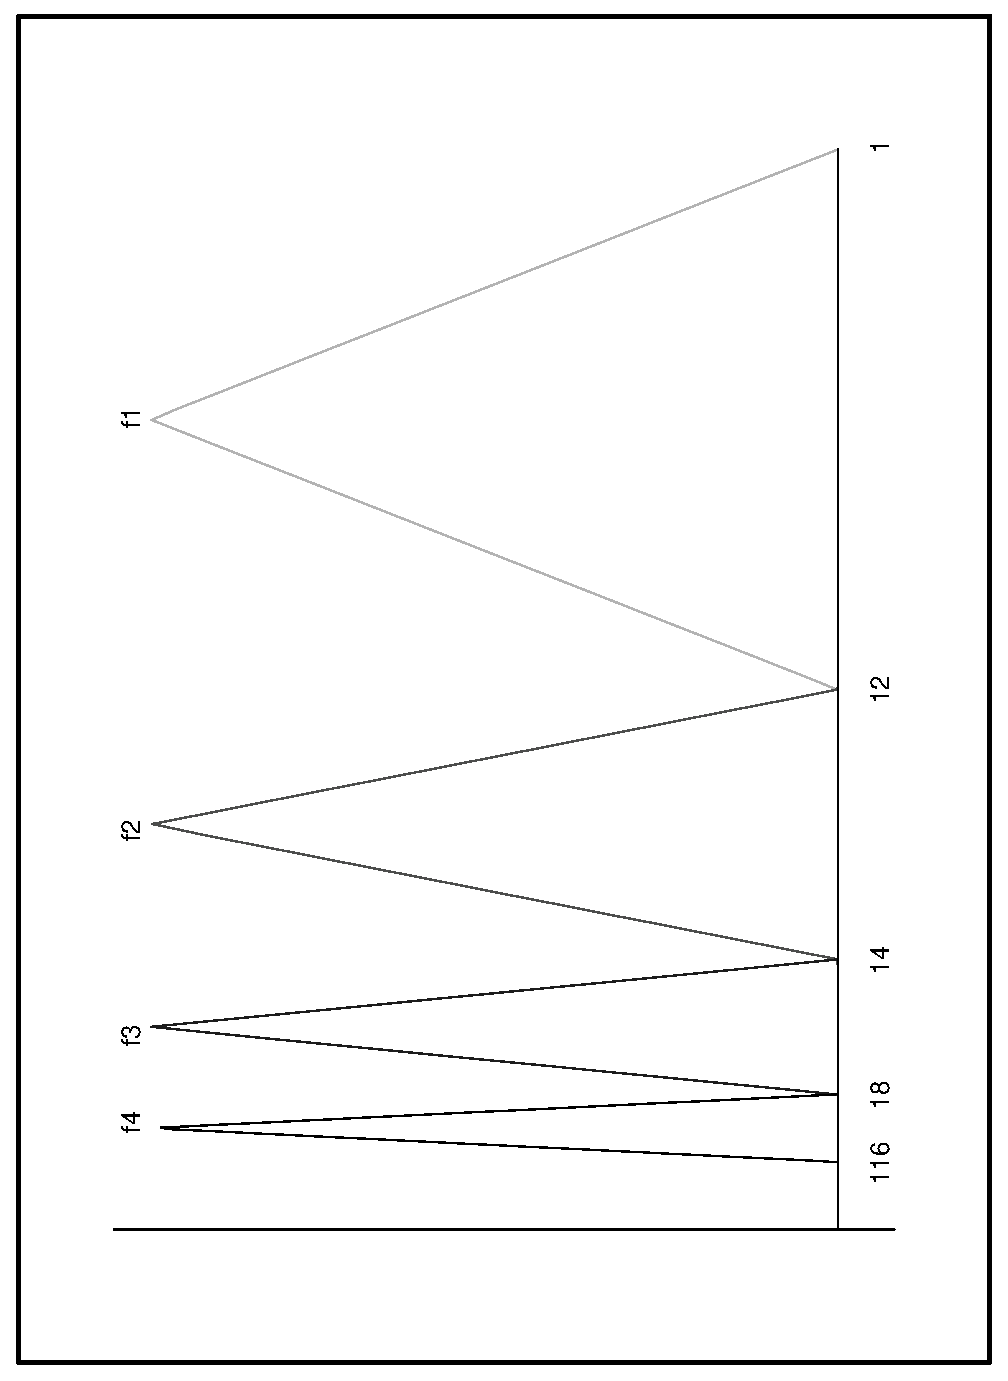
\includegraphics[height=12cm,
    width=7cm,angle=-90]{noprecom.eps}
    \caption{Funciones del Ejemplo
    \ref{ejem,contnopre}}\label{fig,contnopre}
\end{center}
\end{figure}

Puede demostrarse que la distancia de cualquiera de las funciones
de la sucesi\'on a otra es igual a 1. De modo que $f_n\in
\overline{B(0,1)}$. Sea $C:=\{f_n:n\in\nn\}$, observemos que como
subespacio $C$ resulta ser un e.m. discreto, as\'{\i}, por el
Ejemplo anterior y el Ejercicio \vref{ejer,subpreespre},
$\C{B(0,1)}$ no puede ser totalmente acotado.
\end{ejemplo}

Recordemos que, en un e.m. $(X,d)$, una familia de conjuntos
abiertos $\{U_i\}_{i\in I}$ es un \index{\emph{cubrimiento por
abiertos}} de $A\subset X$ si
\[
    A\subset\bigcup\limits_{i\in I}U_i.
\]
\begin{definicion} Un subconjunto $A$ de un e.m. $(X,d)$ se dir\'a
\index{compacto} si, y solo si, todo cubrimiento por abiertos de
$A$ tiene un subcubrimiento finito. Es decir, si $\{U_i\}_{i\in
I}$ es un cubrimiento  de $A$, existe un conjunto finito $F\subset
I$ tal que $\{U_i\}_{i\in F}$ es un cubrimiento.
\end{definicion}



\begin{ejercicio} Demostrar que un eespacio m'etrico discreto es compacto
si, y solo si, es finito.
\end{ejercicio}

\begin{ejercicio} Demostrar que un conjunto totalmente acotado es
acotado.
\end{ejercicio}

\begin{ejercicio}\label{ejer,subpreespre} Demostrar que un
subconjunto de un conjunto totalmente acotado es totalmente
acotado.
\end{ejercicio}

\begin{ejercicio} Demostrar que un conjunto compacto es cerrado y
acotado.
\end{ejercicio}

\begin{ejercicio} Demostrar que si $f:(X,d)\to (Y,d')$ es continua
y $X$ compacto entonces $f(X)$ es compacto. Como corolario
demostrar que si $f:X\to\mathbb{R}$ y $X$ es compacto entonces $f$
alcanza u n m'aximo y un m'inimo.
\end{ejercicio}

\begin{teorema}[Caracterizaci'on de compacidad en espacios m'etricos]
 Sea $(X,d)$ un  espacio m'etrico. Entonces son
equivalentes:

\begin{enumerate}
\item\label{inc,compacto} $X$ es compacto;
\item\label{inc,toacotadoycomp} $X$ es totalmente acotado y
completo.
\item\label{inc,subs} Toda sucesi'on en $X$ tiene una subsucesi'on convergente.
\end{enumerate}
\end{teorema}
\begin{demo} Veamos que
\ref{inc,compacto}$\Rightarrow$\ref{inc,subs}. Por el absurdo
supongamos que existe una sucesi'on $\{a_n\}$ en $X$ que no tiene
ninguna subsucesi'on convergente. Definamos $\Gamma$ como la
colecci'on de todos los conjuntos abiertos $G$ de $X$ tales que
$G$ tiene una cantidad finita de elementos de la sucesi'on, es
decir:
\[
G\in\Gamma\Leftrightarrow \#\{n:a_n\in G\}<\infty.
\]
Vamos a probar que $\Gamma$ es un cubrimiento de $X$. Supongamos
que $x\in X$ y $x\notin G$ para todo $G\in\Gamma$. De modo que,
por definici'on, cada abierto que contiene a $x$ contiene
infinitos t'erminos de la sucesi'on $\{a_n\}$. En particular,
podemos encontrar $n_1$ tal que $a_{n_1}\in B(x,1)$. Ahora podemos
encontrar $n_2>n_1$ tal que $a_{n_2}\in B(x,\frac12)$. Y as'i
continuamos, constru'imos una subsucesi'on $a_{n_k}$ tal que
$a_{n_k}\in B(x,\frac1k)$. Lo que implica que $a_{n_k}$ converge a
$x$.

\end{demo}
